\spacing{1.3}


\section{Introducción}
%Aunque los experimentos de Faraday sobre la electrolisis en 1830 sugirieron que el átomo estaba compuesto por cierto tipo de partículas, no fue hasta finales del siglo
%XIX cuando se comprobó la divisibilidad del átomo y su naturaleza eléctrica.
%Estos avances llegaron con el estudio de las descargas eléctricas sobre tubos de vacío, la radioactividad y los espectros atómicos.
Para estudiar la estructura atómica, es necesario establecer un modelo que nos permita tener una idea general de como está formado y las partes que lo forman, para ello utilizamos lo que conocemos como \azuln{modelo atómico}.
% Así, los rayos catódicos descubiertos en 1886
% por Goldstein, el descubrimiento de los rayos catódicos en 1895 posteriormente identificados por J.J. Thomson como unas partículas cargadas a las que denominadas electrones;la radiactividad natural descubierta por Becquerel (1896), la cual permitió demostrar que todos los elementos químicos tendrán algo en común (partículas positivas, \(\alpha\), partículas negativas , \(\beta\), y radiación de muy alta energía) o el análisis espectroscópico descubierto por Bunsen en 1860 y mejorado por Balmer en 1885, trajeron consigo los primeros intentos por modelar al gran desconocido, el \textbf{átomo}.
% \section{Modelos atómicos}
\vspace{6pt}
\begin{definition}[Modelo atómico]
    Es una representación de la estructura del átomo que intenta explicar su comportamiento y propiedades
\end{definition}
% A l largo de la historia se han ido proponiendo diferentes modelos atómicos. Los principales modelos atómicos propuestos se irán explicando en los siguientes apartados.


\section{Primeros modelos atómicos}

\subsection{Modelo atómico de Dalton}
El modelo atómico de Dalton se basaba en los siguientes postulados:
\begin{itemize}
    \item La materia está formada por partículas denominadas átomos.
    \item Todos los átomos de un mismo elemento son iguales.
    \item Los átomos son partículas muy pequeñas.
    \item Los átomos son partículas indivisibles.
    \item Dos o más átomos son iguales si tienen las mismas propiedades físicas y químicas.
    \item Dos o más átomos pueden unirse cuantitativamente para formar moléculas.
\end{itemize}
%    \begin{figure}[H]
%        \centering
%        \includegraphics[scale=0.3]{images/imagesUD1EstructuraAtomica/UD1_Teoria/dalton_atomic_model}
%        \caption{Modelo atómico de Dalton}
%        \label{fig:modelo_dalton}
%    \end{figure}

\subsection{Modelo de Thomson}\label{subsec:modelo-de-thomson}
Thomson pensaba que los átomos estaban constituidos por partículas más elementales y a raíz del descubrimiento del electrón mediante el experimento con los rayos catódicos postuló que:
\begin{itemize}
    \item El átomo es una masa de protones en las que están incrustados los electrones.
    \item El átomo es neutro, tiene el mismo número de protones como de electrones
\end{itemize}

En este modelo se conoce como \textbf{plum-pudding} donde las cargas positivas estarían repartidas por todo el átomo y las negativas se encontrarían en unas posiciones fijas, pero en número suficiente para que el conjunto resultara neutro.

%    \begin{figure}[H]
%        \begin{subfigure}{0.45\linewidth}
%            \centering
%            \includegraphics[scale=1]{images/imagesUD1EstructuraAtomica/UD1_Teoria/Thomson_model.pdf}
%            %\caption{}
%            %\label{fig:}
%        \end{subfigure}
%        \hfill
%        \begin{subfigure}{0.45\linewidth}
%            \centering
%            \includegraphics[scale=0.5]{images/imagesUD1EstructuraAtomica/UD1_Teoria/thomson_model.jpeg}
%            \caption{Modelo atómico de Thomson}
%            %\label{fig:}
%        \end{subfigure}
%    \end{figure}
Este modelo explica la formación de iones positivos o negativos, la electricidad estática y la corriente eléctrica.
\begin{figure}[H]
    \centering
    \begin{subfigure}[b]{0.45\textwidth}
        \centering
        % [FIGURA ORIGINAL] \includegraphics[scale=0.2]{images/imagesUD1EstructuraAtomica/UD1_Teoria/dalton_atomic_model}
        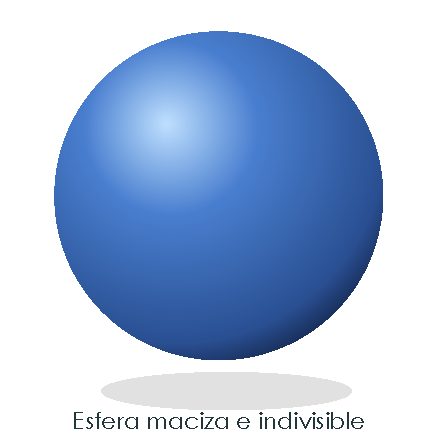
\includegraphics[width=0.75\linewidth]{FigurasSVG/UD1_Estructura_Atomica/pdf/UD1_01_modelo_dalton.pdf}
        \caption{Modelo atómico de Dalton}
        \label{fig:modelo_dalton}
    \end{subfigure}
    \hfill
    \begin{subfigure}[b]{0.45\textwidth}
        \centering
        % [FIGURA ORIGINAL] \includegraphics[scale=0.4]{images/imagesUD1EstructuraAtomica/UD1_Teoria/thomson_model.jpeg}
        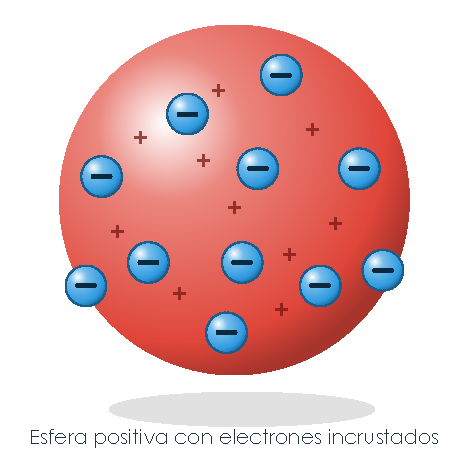
\includegraphics[width=0.8\linewidth]{FigurasSVG/UD1_Estructura_Atomica/pdf/UD1_02_modelo_thomson.pdf}
        \caption{Modelo atómico de Thomsom}
        \label{fig:modelo_thomsom}
    \end{subfigure}
    \caption{Modelos atómicos de Dalton y Thomsom}
    \label{fig:modelos_dalton_thomsom}
\end{figure}

\subsection{Modelo atómico de Rutherford}\label{subsec:modelo-atomico-de-rutherford}

Rutherford propuso el átomo formado por un núcleo y una periferia de electrones girando alrededor de este.
Este modelo se puede basar en los siguientes postulados:
\begin{itemize}
    \item El átomo tiene estructura planetaria.
    \item El átomo posee un núcleo central pequeño, con carga eléctrica positiva y que contiene casi toda la masa del átomo.
    \item Girando en órbitas circulares a grandes distancias alrededor del núcleo hay pequeñas masas con carga eléctrica negativa (los electrones).
    La atracción eléctrica entre los electrones y el núcleo es la fuerza centrípeta que permite a aquellos girar alrededor de este.
    \begin{centeredequation}
        F_e = F_c \Rightarrow K\ \dfrac{Q_n \cdot q_e}{r^2} = m_e\ \dfrac{v_e^2}{r}\label{eq:fuerzelectrica_fuerzacentripeta}
    \end{centeredequation}
    siendo:
    \begin{itemize}
        \item \(K = \text{Constante de Coulomb}\).
        En el vacío \(K = \SI{9e9}{\newton\square\metre\per\square\coulomb}\).
        \item \(Q_n\) es la carga del núcleo y depende del átomo.
        Se puede considerar como \(Q_n = Z\cdot q_e\) siendo \(Z\) el número atómico y como la carga del proton es la misma en valor absoluto que la carga del electrón se puede poner en función de esta.
        \item \(q_e\) es la carga del electrón, cuyo valor es de \qty{1.6e-19}{\coulomb}.
        \item \(r\) el radio de la órbita del electrón.
        \item \(m_e\) es la masa del electrón, cuyo valor es  \qty{9.11e-31}{\kg}
        \item \(v_e\) es la velocidad del electrón.
    \end{itemize}
    \item La suma de las cargas eléctricas negativas de los electrones debe ser igual a la carga positiva del núcleo, ya que el átomo es eléctricamente neutro.
    \item El átomo está prácticamente hueco.
\end{itemize}
\begin{figure}[H]
    \begin{subfigure}[c]{0.45\textwidth}
        \centering
        % [FIGURA ORIGINAL] \includegraphics[scale=0.25]{images/imagesUD1EstructuraAtomica/UD1_Teoria/rutherford_model_c}
        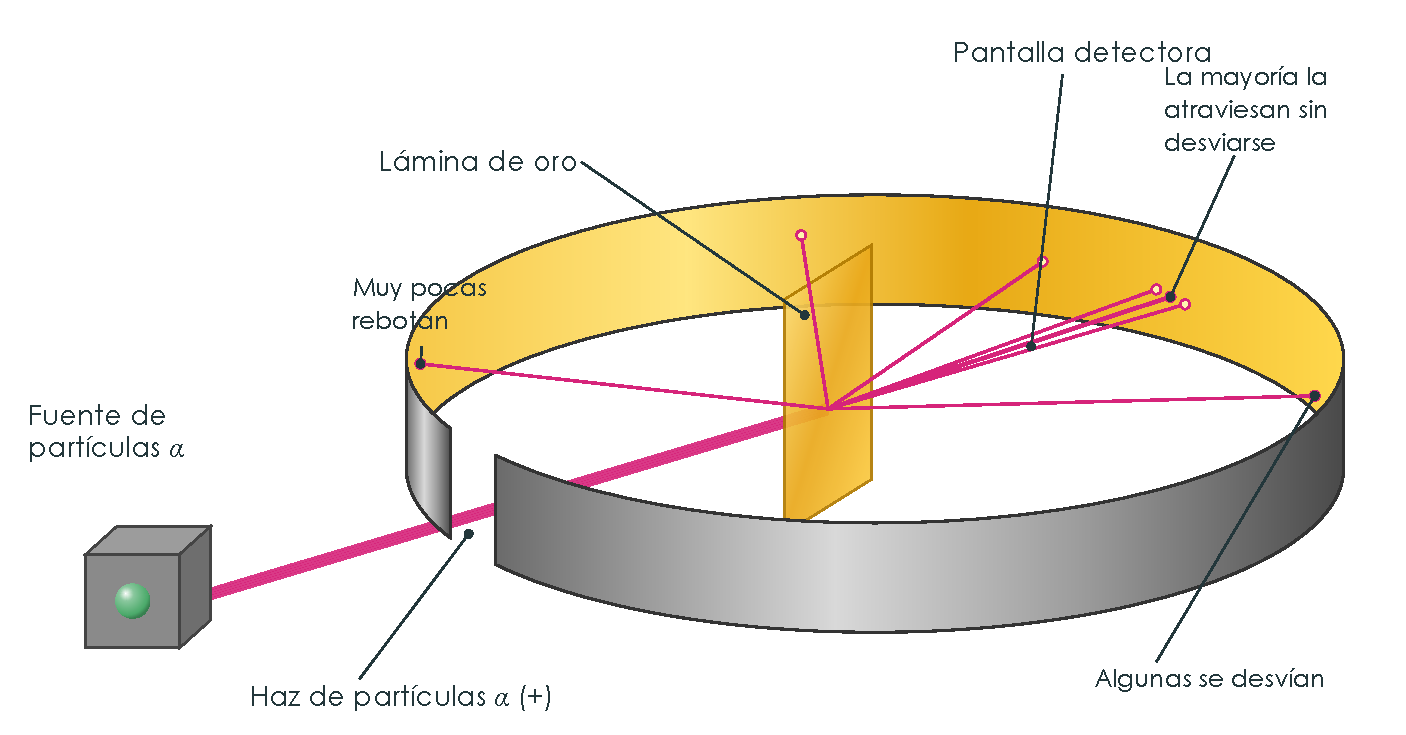
\includegraphics[width=1.0\linewidth]{FigurasSVG/UD1_Estructura_Atomica/pdf/UD1_03_experimento_rutherford.pdf}
        \caption{Experimento de Rutherford}
        \label{fig:experimento_rutherford}
    \end{subfigure}
    \hfill
    \begin{subfigure}[c]{0.45\textwidth}
        \centering
        % [FIGURA ORIGINAL] \includegraphics[scale=0.15]{images/imagesUD1EstructuraAtomica/UD1_Teoria/rutherford_model.png}
        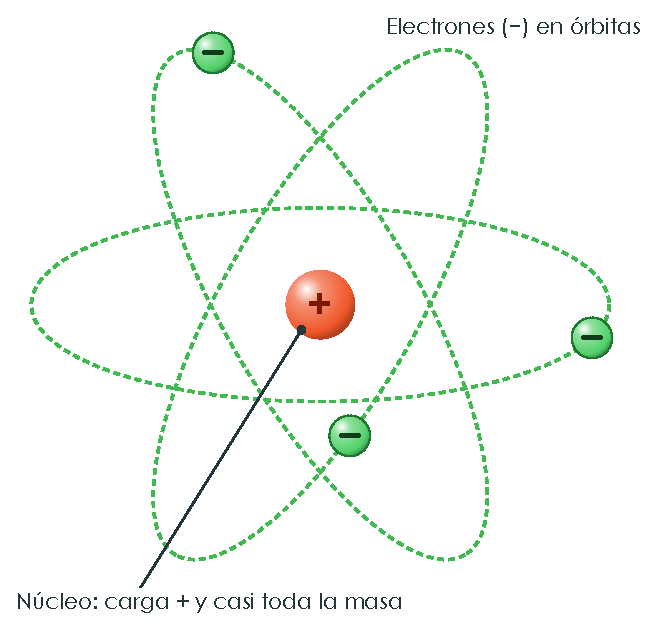
\includegraphics[width=0.85\linewidth]{FigurasSVG/UD1_Estructura_Atomica/pdf/UD1_04_modelo_rutherford.pdf}
        \caption{Modelo atómico de Rutherford}
        \label{fig:modelo_rutherford}
    \end{subfigure}
    \caption{Experimento y modelo atómico de Rutherford}
    \label{fig:experimento_modelo_rutherford}
\end{figure}
Para llegar a estas conclusiones, Rutherford se basó en un experimento donde se hacía pasar partículas cargadas positivamente sobre un alámina de oro. En el experimento de Rutherford, la mayor parte de las partículas atravesaban la lámina del metal sin desviarse, por eso se propuso que el átomo estaba prácticamente hueco.
Solo Una de cada \num{10000} chocaba contra el núcleo y rebotaba (\ref{fig:experimento_rutherford}).

En la figura \ref{fig:modelo_rutherford} tenemos la representación del modelo atómico de Rutherford.

\paragraph{Problemas o defectos del modelo de Rutherford: }

\begin{enumerate}[label=\numberballmDarkTeal]
        \item Una carga acelerada debería emitir ondas electromagnéticas y dicha emisión provocaría la pérdida de energía lo que haría que el electrón describiera órbitas de radio decreciente hasta caer al núcleo.
        \item No daba explicación de los espectros atómicos.
        Según su modelo los espectros serían continuos, algo que no sucede.
        Más adelante veremos lo que son los espectros de absorción y emisión
\end{enumerate}


\section{Nuevos modelos atómicos}\label{sec:nuevos-modelos-atomicos}

\subsection{Modelo atómico de Bohr}\label{subsec:modelo-atomico-de-bohr}

El modelo atómico de Bohr podemos entenderlo siguiendo según los postulados de su modelo:

\begin{enumerate}[label=\numberballmDarkTeal]
        \item Los electrones giran en órbitas estables alrededor del núcleo.
        \item Las únicas órbitas permitidas por el electron son las que cumplen.
        \begin{centeredequation}
            m_e\ v\ r = n\ \dfrac{h}{2\ \pi}
            \label{eq:cuantizacion_energia}
        \end{centeredequation}
        Donde \(\bm{n}\) solo puede tomar valores naturales y hace referencia al nivel energético \(n\) donde \(n\) puede tomar los valores (\(1,2,3,4,5\ \dots\)), \(r\) es el radio de la órbita y  \(h\) la constante de Planck.

        La expresión anterior viene de establecer que el momento angular está cuantizado, es decir depende de números enteros de \(\hslash\).
        Donde:
        \begin{centeredequation}
            L = n\ \hslash \qquad \qquad \text{hay que tener en cuenta que: } \hslash = \dfrac{h}{2\pi}
        \end{centeredequation}
        \item Cuando un electrón pasa de una órbita superior a una órbita inferior, la diferencia de energía se emite en forma de energía electromagnética.

        La emisión o absorción de radiación electromagnética por los átomos se produce en forma de \azuln{cuantos}, unas diminutas cantidades elementales de energía según:
        \begin{centeredequation}
            \Delta E = h\;\nu
        \end{centeredequation}
        Si se produce el proceso inverso, de una órbita inferior a otra superior se absorbe energía.
        En ambos procesos la energía puesta en juego será:
        \begin{centeredequation}
            E_2-E_1 = h\;\nu
        \end{centeredequation}
        Siendo \(E_2\) la energía en la órbita final mientras que \(E_1\) será la energía en la órbita inicial
\end{enumerate}
A partir de los postulados de Bohr podemos calcular:
\begin{enumerate}[label=\letraminuscula]
    % \item \textbf{Velocidad del electrón}. Estableciendo la condición de que el electrón realiza una trayectoria circular alrededor del núcleo tendremos que  $F_c=m\ a_c$. En este caso la fuerza centrípeta será la fuerza eléctrica lo que nos permite llegar a expresión:

    %     \begin{gather*}
    %         F_e = F_c \Rightarrow K\ \dfrac{Z \cdot q_e^2}{r^2} = m_e\ \dfrac{v_e^2}{r}\separ
    %         \kcoulomb\ \dfrac{Z \cdot q_e^2}{r^{\cancelred{2}}} =  m_e\ \dfrac{v_e^2}{\cancelred{r}}
    %     \end{gather*}
    %     despejando la velocidad de la última ecuación obtendríamos que:
    %     \begin{centeredequation}
    %         \tcboxmath[opteqA]{v^2 =  \dfrac{Q_n\  q_e}{m_e\ r}}
    %     \end{centeredequation}

    %     o bien

    %     \begin{centeredequation}
    %         \tcboxmath[opteqA]{v =\sqrt{ \dfrac{Q_n\  q_e}{m_e\ r}}}
    %     \end{centeredequation}
    \item \textbf{Velocidad del electrón}.
    Si tenemos en cuenta la ecuación \eqref{eq:cuantizacion_energia} podemos despejar la velocidad y obtendremos que:
    \begin{centeredequation}
        \tcboxmath[opteqA]{v = n\ \dfrac{h}{m_e\ 2 \pi\ r}}
        \label{eq:velocidad_electron}
    \end{centeredequation}
    \item \textbf{Cálculo del radio de las órbitas}:
    Si tenemos en cuenta la condición de que la fuerza de atracción electrostática entre el núcleo es igual o es la que ejerce de fuerza centrípeta podemos calcular el rádio de la órbita del \el.
    Sabemos que la fuerza electroestática es:
    \begin{centeredequation}
        F_e = K\ \dfrac{Q_n\ q_e}{r^2}
    \end{centeredequation}
    Siendo \(K\) la constante de Coulomb, \(Q_n\) es la carga del núcleo y \(q_e\) la carga del electrón.
    Ya vimos anteriormente que que la carga del núcleo la podemos escribir como \(Q_n = Z\ q_{proton}\) como la carga del protón y la carga del electrón es la misma, podemos decir que \(Q_n = Z\cdot q_e\).
    También sabemos que la fuerza centrípeta tiene la siguiente expresión:
    \begin{centeredequation}
        F_c = m_e\ \dfrac{v_e^2}{r}
    \end{centeredequation}
    Si igualamos la \(F_e\) y la \(F_c\) tendremos que:
    \begin{centeredequation}
        F_e = F_c \Rightarrow K\ \dfrac{Z \cdot q_e^2}{r^2} = m_e\ \dfrac{v_e^2}{r}
        \label{eq:centripeta_electrica}
    \end{centeredequation}
    y la ecuación \eqref{eq:velocidad_electron}, tras simplificar términos y despejar el radio llegamos a la expresión del radio.
    \begin{centeredequation}
        \begin{aligned}
            % F_e = F_c \Rightarrow K\ \dfrac{Q_n \cdot q_e}{r^2} = m_e\ \dfrac{v_e^2}{r}\separ
            K\ \dfrac{Q_n \cdot q_e}{r^2} = m_e\ n^2\ \dfrac{h^2}{4\pi^2\ m_e^2 \ r^3}\notag\separ
            \tcboxmath[opteqA]{r = n^2\ \dfrac{h^2}{4\pi^2\ m_e\ K\ Z\ q_e^2}}
        \end{aligned}
    \end{centeredequation}
    Debido a que \(h, m_e, K, q_e\) son constantes, podemos agruparlos en una nueva constante, denominada \(a\), que se corresponde al radio de la primera órbita de Bohr
    \begin{centeredequation}
        a = \dfrac{h^2}{4\pi^2\ m_e\ K\ Z\ q_e^2}
    \end{centeredequation}
    Por lo tanto, el radio de la órbita será:
    \begin{centeredequation}
        \tcboxmath[opteqA]{r = a\ n^2}
    \end{centeredequation}
    \item \textbf{Cálculo de la energía del electrón}: La energía total del electrón será la suma de la energía potencial eléctrica y la energía cinética debido al movimiento.
    \begin{centeredequation}
        E_T = E_p + E_c = -\kcoulomb\; \dfrac{Z\ q_e^2}{r} + \dfrac{1}{2}\; m_e\ v^2
        \label{eq:energiatotal}
    \end{centeredequation}
    De la ecuación \eqref{eq:centripeta_electrica} se deduce que:
    \begin{centeredequation}
        m_e\ v_e^2 = K\dfrac{Z\ q_e^2}{r}
    \end{centeredequation}
    Si esta última expresión la sustituimos en la ecuación \eqref{eq:energiatotal} tenemos que:
    \begin{centeredequation}
        E_T = -\dfrac{1}{2}\ K\ \dfrac{Z\ q_e^2}{r}
    \end{centeredequation}
    como \(K\) y \(q_e\) son constantes y como \(r = a\ n^2\) podemos escribir la última expresión como:
    \begin{centeredequation}
        E_T = -\dfrac{1}{2}\ K\ \dfrac{Z\ q_e^2}{a\ n^2} = - b \ \dfrac{1}{n^2}
    \end{centeredequation}
    siendo \(b = \dfrac{1}{2}\ K \dfrac{Q_n\ q_e}{a}\) quedando por tanto la energía total del electrón como:
    \begin{centeredequation}
        \tcboxmath[opteqA]{E_T = - b  \dfrac{1}{n^2}}
    \end{centeredequation}
    La constante \(\bm{b}\) coincide con el valor absoluto de la \textbf{energía de la primera órbita de Bohr} (\(n=1\)), que en el caso del átomo de hidrógeno tiene un valor de \energia[j]{-2.18e-18} que equivalen a unos \energia[ev]{-13.6} ( \(\SI{1}{\electronvolt} =  \SI{1.6e-19}{\joule} \)).

    Por convenio de signos, el valor negativo significa que se trata de una \textbf{energía de estabilización}
    % Si en esta expresión se sustituye el valor de la velocidad y luego sustituimos el valor de $r$ la energía tendrá la forma:
    % \begin{centeredequation}
    %     E_T = -\dfrac{1}{n^2}\; \dfrac{m_eZ^2q_e^4}{8h^2\varepsilon_0^2}
    % \end{centeredequation}
    % Si al conjunto de todas estas constantes se engloba en una sola tendremos que
    % \begin{centeredequation}
    %     E_T = -\dfrac{1}{n^2}\;K^\prime
    % \end{centeredequation}
    \item \textbf{Cálculo de la diferencia de energía asociada entre dos órbitas}: Si un electrón pasa de una órbita $n_1$ a $n_2$ la variación de energía vendrá dada por:
    \begin{centeredequation}
        \Delta E = E_{2} - E_1 = b\ \left[\dfrac{1}{n_1^2} - \dfrac{1}{n_2^2} \right]
    \end{centeredequation}
    Si aplicamos que: $\Delta E = h\; \nu  \Rightarrow E_2-E_1 = h\; \nu \Rightarrow E_2-E_1= h\ \dfrac{c}{\lambda}$ tendremos que
    \begin{centeredequation}
        \Delta E = E_2 - E_1 =  b\  \biggl( \dfrac{1}{n_1^2} - \dfrac{1}{n_2^2} \biggr)  = h\ \dfrac{c}{\lambda}
    \end{centeredequation}
    despejando \(\dfrac{1}{\lambda}\) obtenemos la ecuación espectral derivada de la teoría de Bohr:
    \begin{centeredequation}
        \dfrac{1}{\lambda} = \dfrac{b}{h\ c}\biggl( \dfrac{1}{n_1^2} - \dfrac{1}{n_2^2} \biggr)
    \end{centeredequation}
    Ahora podemos comprobar que el factor constante, es decir \(\frac{b}{h\ c}\) es igual a la constante de Rydberg (ver ecuación \eqref{eq:ecucion_rydberg}. Para el átomo de hidrógeno:
    \begin{centeredequation}
        \dfrac{b}{h\ c} = \dfrac{\num{2.18e-18}}{\num{6.63e-34}\cdot \num{3e8}} = \SI{1.096e7}{\metre^{-1}}
    \end{centeredequation}
    % Si agregamos todas las constantes en una única constante $K^{\prime\prime}$
    % \begin{centeredequation}
    %     \nu = K^{\prime\prime}\; \left[\dfrac{1}{n_1^2} - \dfrac{1}{n_2^2} \right]
    % \end{centeredequation}
    % Si recordamos que $c = \lambda\;\nu$ se puede obtener la expresión:
    % \begin{centeredequation}
    %     \dfrac{1}{\lambda} = \dfrac{\nu}{c}= \dfrac{K^{\prime\prime}}{c}\; \left[\dfrac{1}{n_1^2} - \dfrac{1}{n_2^2} \right]
    % \end{centeredequation}
    % Si agrupamos todas las constantes en un única constante $R$ llamada contante de Rydberg tendremos que:
    % \begin{centeredequation}
    %     \tcboxmath[opteqA]{\dfrac{1}{\lambda} = R\; \left[\dfrac{1}{n_1^2} - \dfrac{1}{n_2^2} \right]}
    % \end{centeredequation}
    % Dando valores a $n_1$ y $n_2$ se obtienen las longitudes de onda de las series espectrales del hidrógeno (Lyman, Balmer, Paschen, Brackett, Pfund)
\end{enumerate}
De manera esquemática, el modelo atómico de Bohr lo podemos ver tal y como se muestra en la la Figura \ref{fig:modelo_bohr}
\begin{figure}[H]
    \centering
    % [FIGURA ORIGINAL] \includegraphics[scale=0.3]{images/imagesUD1EstructuraAtomica/UD1_Teoria/modelo_bohr.jpeg}
    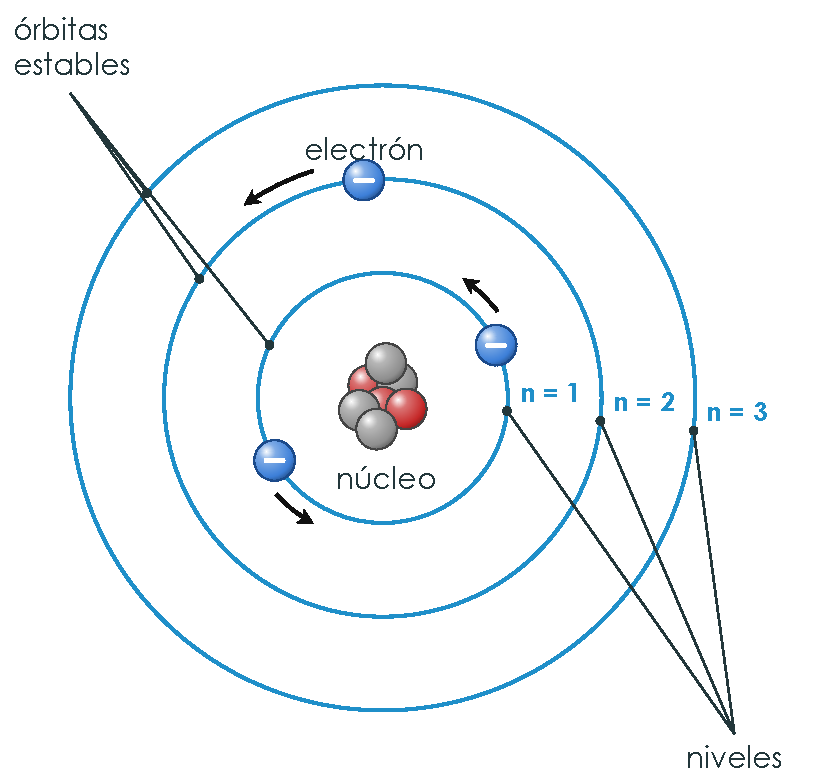
\includegraphics[width=0.5\linewidth]{FigurasSVG/UD1_Estructura_Atomica/pdf/UD1_05_modelo_bohr.pdf}
    \caption{Modelo atómico de Bohr}
    \label{fig:modelo_bohr}
\end{figure}

\paragraph{Aciertos del modelo de Bohr}
\begin{enumerate}[label=\numberballmDarkTeal]
        \item Permite deducir los radios de las órbitas.
        \item Permite deducir la fórmula que Balmer y Rydberg hallaron empíricamente.
        \item Esta deducción teórica proporciona unos valores de frecuencias y energías muy acordes con los hallados experimentalmente por los espectroscopístas.
\end{enumerate}
\paragraph{Limitaciones del modelo de Bohr}
\begin{enumerate}[label=\numberballmDarkTeal]
        \item Supone que las órbitas son circulares y no elípticas.
        \item Solo es aplicable de manera estricta al átomo de hidrógeno.
        \item Los avances en espectroscopia mostraron nuevas rayas que no se pueden explicar con este modelo.
\end{enumerate}

\subsection{Modelo atómico de Sommerfeld (Bohr-Sommerfeld)}

A medida que se iban mejorando las técnicas espectroscópicas, se fueron observando que las líneas espectrales eran en realidad \textbf{multipletes} es decir varias rayas juntas.
\begin{figure}[H]
    \centering
    % [FIGURA ORIGINAL] \includegraphics[scale=0.65]{images/imagesUD1EstructuraAtomica/UD1_Teoria/multipletes.PNG}
    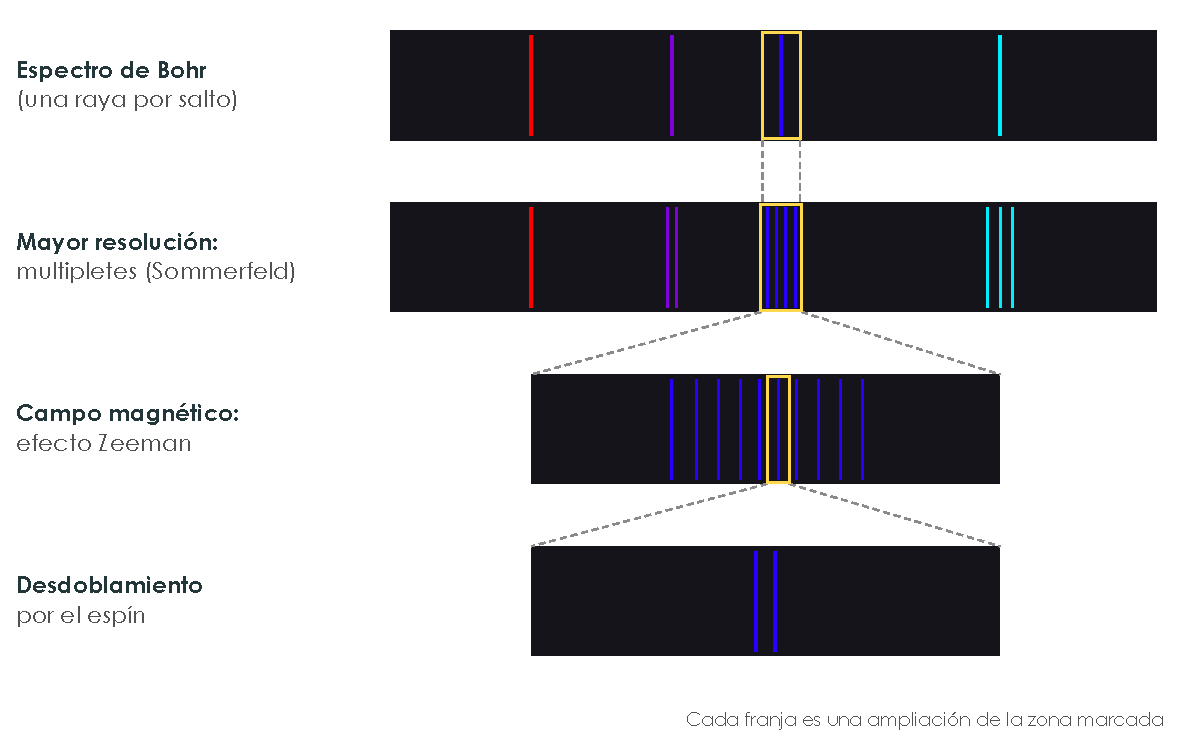
\includegraphics[width=0.7\linewidth]{FigurasSVG/UD1_Estructura_Atomica/pdf/UD1_06_multipletes.pdf}
    \caption{Desdoblamiento de las líneas espectrales}
    %\label{fig:}
\end{figure}
Sommerfeld propuso como explicación que cada órbita de Bohr, es decir cada nivel constaba en realidad de varias órbitas, o más exactamente de varios tipos de órbitas, que se diferenciaban en la forma en la que los electrones orbitaban alrededor del núcleo.
Supuso que siempre habría una órbita circular pero también órbitas elípticas con el núcleo situado en sus focos.

Matemáticamente, estas órbitas se representaban mediante un nuevo número cuántico  \(\bm{l}\) o también \(\bm{m_l}\) denominado \textbf{número cuántico secundario} o \textbf{azimutal}.
Los posibles valores se \(l\) van desde \(0 ... n-1\).
\begin{table}[H]
    \centering
    \caption{Nombre de los orbitales}
    \vspace{-5pt}
    \begin{tabular}{@{}ccc@{}}
        \toprule
        \textbf{Nº Cuántico} & \textbf{Orbital} & \textbf{Nombre} \\
        \bottomrule
        0                    & \(\bm{s}\)       & sharp \\[3pt]
        1                    & \(\bm{p}\)       & principal              \\[3pt]
        2                    & \(\bm{d}\)       & diffuse \\[3pt]
        3                    & \(\bm{f}\)       & fundamental     \\
        \bottomrule
    \end{tabular}
    \label{tab:nombre_orbitales}
\end{table}
%\begin{table}[H]
%    \centering
%    \begin{tblr}{
%        colspec = {Q[c,m]|Q[c,m]|Q[c,m]},
%        row{1} = {bg=mybluecolour, fg = white, font=\sffamily},
%        vlines = {1}{white},
%    }
%        \hline
%        \textbf{Nº. cuántico \(l\)} & \textbf{Órbita} & \textbf{Nombre} \\
%        \hline
%        0                           & \(\bm{s}\)      & sharp           \\
%        \hline
%        1                           & \(\bm{p}\)      & principal       \\
%        \hline
%        2                           & \(\bm{d}\)      & diffuse         \\
%        \hline
%        3                           & \(\bm{f}\)      & fundamental     \\
%        \hline
%    \end{tblr}
%\end{table}

\subsection{Modelo mecano-cuántico ondulatorio}

\textbf{Erwin Schrödinger} describió al electrón como una onda vibrando alrededor del núcleo y que estaba a su vez en todos los puntos de la órbita.

\begin{figure}[H]
    \centering
    % [FIGURA ORIGINAL] \includegraphics[scale=0.7]{images/imagesUD1EstructuraAtomica/UD1_Teoria/onda_atomo.PNG}
    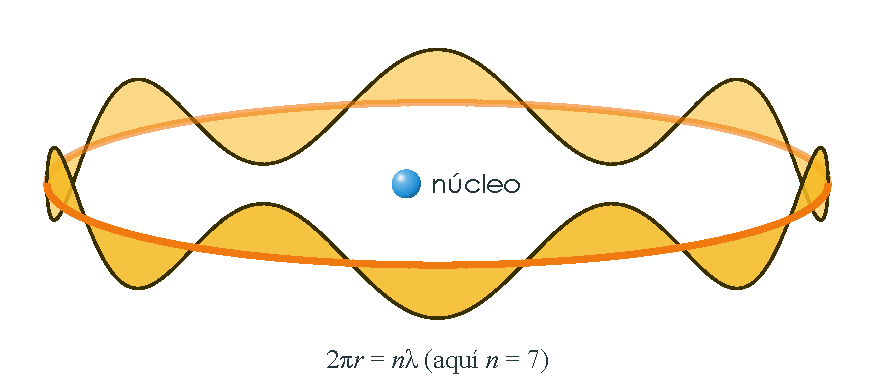
\includegraphics[width=0.6\linewidth]{FigurasSVG/UD1_Estructura_Atomica/pdf/UD1_07_onda_electron.pdf}
    \caption{}
    %\label{fig:}
\end{figure}
Schrödinger desarrolló una ecuación diferencial para obtener la función de onda \( \Psi \).
\begin{centeredequation}
    \dfrac{\delta^2\Psi}{\delta x^2} + \dfrac{\delta^2\Psi}{\delta y^2} + \dfrac{\delta^2\Psi}{\delta z^2} + \dfrac{8\pi^2m}{h^2}\;(E-V)\;\Psi = 0
\end{centeredequation}
\begin{enumerate}[label=\numberballmDarkTeal]
        \item $\Psi$ es la función de onda y no tiene por sí misma significado físico pero contiene información de la posición del electrón.
        Se le denomina también \blueremark{orbital}.
        \item El cuadrado de la función de onda $|\Psi|^2$ es la \textbf{densidad de probabilidad relativa del electron} y representa la probabilidad de encontrar al electrón en un punto del espacio de coordenadas $(x, y, z)$
        \item \textbf{E}, la energía total del electrón.
        \item \textbf{V}, energía potencial el electrón.
\end{enumerate}
\begin{figure}[H]
    \centering
    % [FIGURA ORIGINAL] \includegraphics[scale=0.9]{images/imagesUD1EstructuraAtomica/UD1_Teoria/funciondeonda_distancia.PNG}
    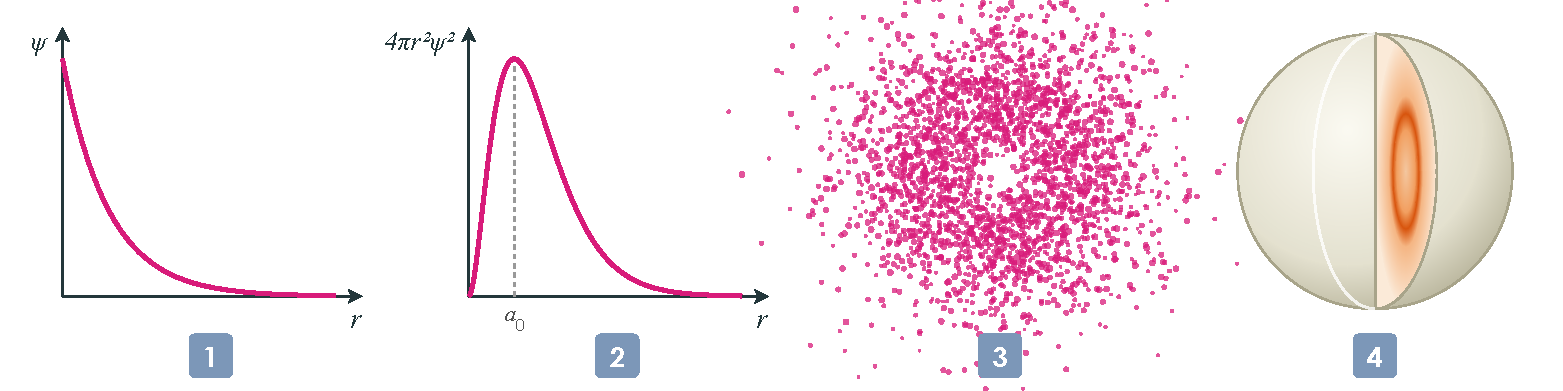
\includegraphics[width=1.0\linewidth]{FigurasSVG/UD1_Estructura_Atomica/pdf/UD1_08_funcion_onda_1s.pdf}
    \caption{1. Función de onda frente la distancia con el núcleo. 2. Probabilidad de encontrar a un electrón frente a la distancia con el núcleo. 3. La probabilidad de encontrar al electrón en diferentes momentos. 4. Estructura espacial del orbital \(\bm{s}\)}
    %\label{fig:}
\end{figure}
Llegados a este punto, es importante conocer perfectamente el significado de órbita y de orbital.
\begin{itemize}
    \item \textbf{Órbita}: línea que describe el electrón en su movimiento alrededor del núcleo (Modelo de Bohr).
    \item \textbf{Orbital}: región en el espacio en la que hay probabilidad superior al 90\% de encontrar al electrón (Modelo mecánico ondulatorio)
\end{itemize}
% \subsubsection{Efecto Compton}

% Arthur Holly Compton, descubrió que algunos rayos X, al dispersarse a través de la materia, perdían energía y en consecuencia su longitud de onda aumentaba. La relación matemática entre la longitud de onda incidente y la resultante es:
% \begin{centeredequation}
%     \tcboxmath[opteqA]{\lambda = \lambda_0 + \; \dfrac{h}{m_e c}\; (1-\cos\theta)}
% \end{centeredequation}
% Donde:
% \begin{gather}
%     \lambda = \text{longitud de onda dispersada}\\\notag
%     \lambda_0 = \text{longitud de onda incidente}\\\notag
%     h = \text{constante de Plank }\SI{6,626e-34}{\joule\s}\\\notag
% \end{gather}

% \begin{gather}
%     m_e = \text{masa del electrón }\SI{9,109e-31}{\kilo\g}\\\notag
%     c = \text{velocidad de la luz } \SI{2,988e8}{\meter\per\s}\\\notag
%     \theta = \text{ángulo de dispersión}
% \end{gather}


\section{Bases experimentales de la mecánica cuántica}

Para entender los nuevos modelos atómicos indicados anteriormente, es necesario conocer algunas de las bases físicas que llevaron a su formulación

\subsection{Teoría de Planck}\label{subsec:teoria-de-planck}

Planck llegó a la conclusión de que la radiación electromagnética (luz) no es un continuo, sino que se emite en forma de pequeños \textbf{paquetes} de energía, llamados cuantos de radiación o \textbf{fotones} cuya energía dependía de la frecuencia de la radiación según la ecuación.
\begin{definition}[Fotón]
    es un \textbf{cuanto} de radiación electromagnética o \textbf{cuanto de energía} y se trata de una partícula de energía en estado puro, que no tiene masa según la siguiente ecuación:
    \begin{centeredequation}
        E = h\ \nu\label{eq:energia_relativista}
    \end{centeredequation}
    Siendo \(h\) la constante de Planck cuyo valor es \SI{6.63e-34}{\joule\s} y \(\nu\) la frecuencia de la radiación.
\end{definition}

La teoría de Planck es muy importante porque marca el inicio de la mecánica cuántica.

La energía de un fotón depende de su frecuencia: cuanto mayor sea esta mayor será la energía que transporta. Sabemos que la frecuencia está relacionada con la longitud de onda según la expresión:
\begin{centeredequation*}
    c = \lambda\ \nu \longrightarrow \nu = \dfrac{c}{\lambda}
\end{centeredequation*}
Si lo sustituimos en la ecuación \eqref{eq:energia_relativista} tendremos que:

\begin{centeredequation}
    E = h\ \dfrac{c}{\lambda}
\end{centeredequation}

La \textbf{energía} de una radiación es la energía de cada uno de sus fotones, mientras que su \textbf{intensidad} viene determinada por el número de fotones.

La \textbf{frecuencia} (\(\nu\)) se mide en \unit{\hertz} (hercios), que equivale a \(1/\unit{\s}\), \si{\s^{-1}} o ciclos/s.

La \textbf{longitud de onda} (\(\lambda\)) se mide en unidades de longitud, como en \unit{\metre}, \unit{\nano\metre} o \unit{\angstrom} que equivale a \SI{e-10}{\metre}.

\subsection{Efecto fotoeléctrico}\label{subsec:efecto-fotoelectrico}

El efecto fotoeléctrico consiste en irradiar un material con una fuente de luz (onda).
La energía de la onda incidente se utiliza para arrancar y acelerar los electrones del material, siendo normalmente el material un compuesto metálico.

\begin{definition}[Energía umbral o trabajo de extracción]
    Se representa con (\(W_0\)) o \( E_0 \) y es la energía justa para arrancar el electrón del metal, también se denomina \textbf{función de trabajo}, \textbf{trabajo de extracción} o \textbf{trabajo umbral} y es característica de cada metal o elemento.
\end{definition}

La energía aplicada durante el efecto fotoeléctrico sería igual a esa energía umbral o función de trabajo y la energía cinética máxima adquirida por dicho electrón.
El balance energético quedaría como:
\begin{centeredequation}
    E = W_0 + E_c\label{eq:efecto_fotoelectrico}
\end{centeredequation}
\begin{centeredequation}
    h\;\nu = W_0 + \dfrac{1}{2}\; m_e\; v_e^2 \label{eq:efecto_fotoelctrico_desarrollado}
\end{centeredequation}

\begin{consejo}[\textbf{Resolución de ejercicios sobre Efecto fotoeléctrico}]
    \phantom{a}

    \begin{enumerate}
        \item Debemos tener en cuenta que el trabajo umbral, también se llama función de trabajo o energía umbral y se representa con \(W_0\).
        \item Esta energía umbral, tendrá también una expresión del tipo: \(W_0 = h\cdot \nu_0\) donde \(\nu_0\) es la frecuencia que se necesita para arrancar un electrón.
        \item Debemos recordar que \(\nu_0\) se relaciona la longitud de onda (\(\lambda_0\)) según la expresión \(c = \lambda_0 \cdot \nu_0\).
        \item La energía \(E\) de la ecuación es la energía de la radiación incidente, si esa energía \(E < W_0 \) no se arrancará ningún electrón.
        \item Cuando me pidan la energía necesaria para arrancar un electrón me están pidiendo esa energía umbral o trabajo umbral.
        \item Si me dan la longitud onda o frecuencia ya sea de la radiación incidente o de la energía umbral me están dando la energía incidente o la energía umbral, ya que la podemos calcular según la ecuación: \( E = h\ \nu \) (ecuación \eqref{eq:energia_relativista}).
        \item La ecuación del efecto fotoeléctrico (ecuación \eqref{eq:efecto_fotoelectrico}) nos dice que cuando se hace incidir una radiación de una determinada energía, esta energía primero se utilizará para arrancar el electrón y si sobra energía es decir si la energía incidente es mayor que la energía umbral, lo que sobra de energía se transforma en energía cinética haciendo que el electrón adquiera una cierta velocidad.
    \end{enumerate}
\end{consejo}

A continuación veamos un posible ejemplo.

\begin{example}
    Calcula la frecuencia umbral y el trabajo de extracción del metal sodio, expresado en electronvoltios (\unit{\electronvolt}), sabiendo que al incidir sobre una superficie de dicho metal una radiación electromagnética cuya frecuencia es de \SI{1.18e15}{\hertz}, los electrones son arrancados con una energía cinética máxima de \energia[j]{4.18e-19}.
    Determina la velocidad máxima a la que salen los electrones.

        {\large{\negsubro{Solución:}}}

    Para evitar errores de cálculos, lo primero que debemos hacer es pasar todas unidades de las magnitudes a las correspondientes unidades del sistema internacional.

    Debemos recordar que el \si{\electronvolt} es una unidad de energía y por tanto debemos pasarla a \si{\joule}, el \si{\hertz} ya está en la unidad del sistema internacional porque equivale a \si{1\per\s}.

    En este caso como podemos ver, todo está en las unidades del sistema internacional.
    Lo primero que haremos es poner la fórmula del efecto fotoeléctrico donde \( E = W_0 + E_c\).
    Como nos piden que obtengamos el trabajo de extracción lo que debemos hacer es despejar \(W_0\) y calcularlo:
    \begin{centeredequation}
        W_0 = E - E_c \rightarrow W_0 = h\ \nu - E_c =  (\num{6.62e-34}\cdot \num{1.18e15}) - \num{4.18e-19} \rightarrow W_0= \SI{3.64e-19}{\joule}
    \end{centeredequation}
    Como nos pide el trabajo de extracción en \unit{\electronvolt} lo que hacemos ahora es hacer el correspondiente cambio de unidades.
    \begin{centeredequation}
        \SI{3.64e-19}{\joule} \cdot \dfrac{\SI{1}{\electronvolt}}{\SI{1.6e-19}{\joule}} = \SI{2.28}{\electronvolt}
    \end{centeredequation}
    Ahora nos pide que calculemos la frecuencia umbral, si sabemos que \(W_ 0 = h\ \nu_0\) tan solo tenemos que despejar \( \nu_0 \) obteniendo que:
    \begin{centeredequation}
        \nu_0 = \dfrac{W_0}{h} \rightarrow \nu_0 = \dfrac{\num{3.64e-19}}{\num{6.63e-34}} \rightarrow \nu_0 = \SI{5.49e14}{\hertz}
    \end{centeredequation}
    También nos piden que calculemos la velocidad máxima de ese electrón, para ello sacaremos la velocidad de la energía cinética ya que nos dan su valor:
    \begin{gather*}
        E_c = \dfrac{1}{2}\ m_e \ v_e^2\separ
        v= \sqrt{\dfrac{2\ E_c}{m_e}} = \sqrt{\dfrac{2\cdot \num{4.18e-19}}{\num{9.1e-31}}} = \velocidad[ms]{9.6e5}
    \end{gather*}
    Quedando, por tanto, las soluciones como:
    \begin{centeredequation}
        \tcboxmath[opteqA]{W_0= \SI{4.88}{\electronvolt}} \qquad \tcboxmath[opteqA]{\nu_0= \SI{1.18e15}{\hertz}} \qquad \tcboxmath[opteqA]{v = \SI{9.6e5}{\mps}}
    \end{centeredequation}
\end{example}

\subsection{Espectros de absorción y de emisión}\label{subsec:espectros-de-absorcion-y-de-emision}

Los espectros de absorción o emisión se producen cuando existe la promoción de un electrón desde un orbital a otro.
Si durante este proceso se emite energía, tendremos un espectro de emisión y si absorbe energía tendremos un espectro de absorción.
\begin{itemize}
    \item \textbf{Espectros de absorción}: Se analiza la radiación absorbida por una muestra.
    Para ello se ilumina la muestra con una radiación compleja, por ejemplo luz blanca y luego se analiza la radiación obtenida tras irradiar la muestra.
    Los átomos de la muestra habrán absorbido algunas radiaciones (alguna parte del espectro electromagnético) y, por tanto, los electrones pasarán de un nivel inferior a otro nivel superior, puesto que ganan energía.
    Estas transiciones se observan con unas líneas negras que indican ese tránsito. Ver Figura \ref{fig:absorcion_atomica}
%        \begin{figure}[H]
%            \centering
%            \includegraphics[scale=0.8]{images/imagesUD1EstructuraAtomica/UD1_Teoria/espectroelectromagnetico.PNG}
%            %\caption{}
%            %\label{fig:}
%        \end{figure}


%        \begin{figure}[H]
%            \centering
%            \includegraphics[scale=1]{images/imagesUD1EstructuraAtomica/UD1_Teoria/espectro_absorcion.PNG}
%            %\caption{}
%            %\label{fig:}
%        \end{figure}
    \item \textbf{Espectros de emisión}: en este caso se analiza la radiación emitida por una muestra sobre la cual no incide ninguna radiación externa. Algunos átomos emiten radiación de forma espontánea como sucede con los cuerpos fluorescentes mientras que los que no lo hacen tienen que ser excitados con una fuente de calor o eléctrica. Las emisiones de estos átomos se verán como unas líneas de color sobre un fondo negro indicando el paso de los electrones dese un nivel superior a un nivel inferior emitiendo, por tanto, energía. Ver Figura \ref{fig:emision_atomica}
%        \begin{figure}[H]
%            \centering
%            \includegraphics[scale=1]{images/imagesUD1EstructuraAtomica/UD1_Teoria/espectro_emision.PNG}
%            %\caption{}
%            %\label{fig:}
%        \end{figure}
\end{itemize}

\begin{figure}[H]
    \centering
    \begin{subfigure}[b]{0.45\textwidth}
        \centering
        % [FIGURA ORIGINAL] \includegraphics[scale=0.75]{images/imagesUD1EstructuraAtomica/UD1_Teoria/espectro_absorcion_atomica}
        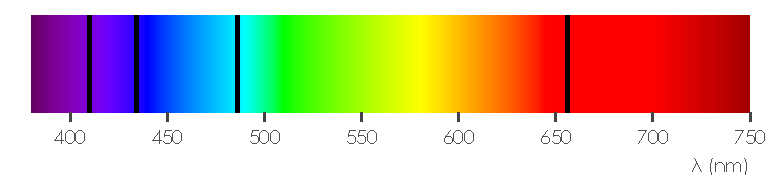
\includegraphics[width=1.0\linewidth]{FigurasSVG/UD1_Estructura_Atomica/pdf/UD1_09_espectro_absorcion_hidrogeno.pdf}
        \caption{Espectro de absorción atómica}
        \label{fig:absorcion_atomica}
    \end{subfigure}
    \hfill
    \begin{subfigure}[b]{0.45\textwidth}
        \centering
        % [FIGURA ORIGINAL] \includegraphics[scale=0.75]{images/imagesUD1EstructuraAtomica/UD1_Teoria/espectro_emision_atomica}
        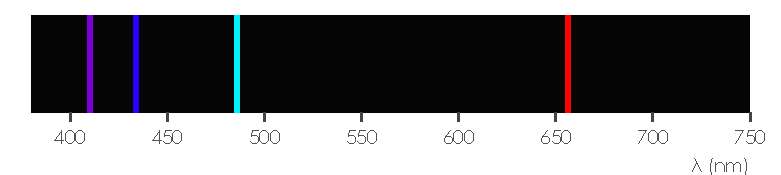
\includegraphics[width=1.0\linewidth]{FigurasSVG/UD1_Estructura_Atomica/pdf/UD1_10_espectro_emision_hidrogeno.pdf}
        \caption{Espectro emisión atómica}
        \label{fig:emision_atomica}
    \end{subfigure}
    \caption{Espectros de emisión y abosrción atómica}
    \label{fig:emision_absorcion_atomica}
\end{figure}

\subsection{Series espectrales}

Las rayas obtenidas en los espectros de emisión y absorción podían obtenerse mediante una ecuación general llamada \textbf{fórmula de Rydberg}:
\begin{centeredequation}
    \dfrac{1}{\lambda} = R\ \biggl(\dfrac{1}{n_1^2} - \dfrac{1}{n_2^2} \biggr) \label{eq:ecucion_rydberg}
\end{centeredequation}
Siendo \(R\) la \textbf{constante de Rydberg} y tiene un valor de \SI{10967756,6}{\metre^{-1}} para el átomo de hidrógeno y \(n_1\) y \(n_2\) son los niveles energéticos en los que se producen el tránsito electrónico.
Son siempre números enteros que van desde el 1 hasta el 7.
El nivel energético menor siempre se asigna al \(n_1\) mientras que el nivel energético mayor a \(n_2\) ya que de la ecuación de Rydberg obtenemos la longitud de onda y esta debe ser siempre positiva.
Si tenemos un espectro de emisión, entonces le pondremos un signo negativo a la energía (desprende energía) y si tenemos un espectro de absorción le pondremos un signo positivo a la energía (absorbe energía).

Tenemos principalmente 4 series espectrales cuyas fórmulas de Rydberg son las siguientes.
\vspace{-8pt}
\begin{multicols}{2}
    \begin{itemize}
        \item \textbf{Serie de Lyman}: \( \dfrac{1}{\lambda} = R\ \biggl(\dfrac{1}{1^2} - \dfrac{1}{n_2^2} \biggr)\)
        \item  \textbf{Serie de Balmer}: \( \dfrac{1}{\lambda} = R\ \biggl(\dfrac{1}{2^2} - \dfrac{1}{n_2^2} \biggr)\)
        \item  \textbf{Serie de Paschen}: \( \dfrac{1}{\lambda} = R\ \biggl(\dfrac{1}{3^2} - \dfrac{1}{n_2^2} \biggr)\)
        \item  \textbf{Serie de Brackett}: \( \dfrac{1}{\lambda} = R\ \biggl(\dfrac{1}{4^2} - \dfrac{1}{n_2^2} \biggr)\)
        \item \textbf{Serie de Pfund}: \( \dfrac{1}{\lambda} = R\ \biggl(\dfrac{1}{5^2} - \dfrac{1}{n_2^2} \biggr)\)
    \end{itemize}
\end{multicols}
Como podemos ver en las fórmulas la serie de Lyman, siempre parte o llega al nivel energético \(n = 1\), la de Balmer a \(n = 2\), la de Paschen a \(n = 3\), la de Brackett a \(n = 4\) y la de Pfund a \(n = 5\).
Estas series espectrales las podemos ver en la Figura \ref{fig:series_espectrales}.

\begin{figure}[H]
    \centering
    % [FIGURA ORIGINAL] \includegraphics[scale=1]{images/imagesUD1EstructuraAtomica/UD1_Teoria/series_espectrales}
    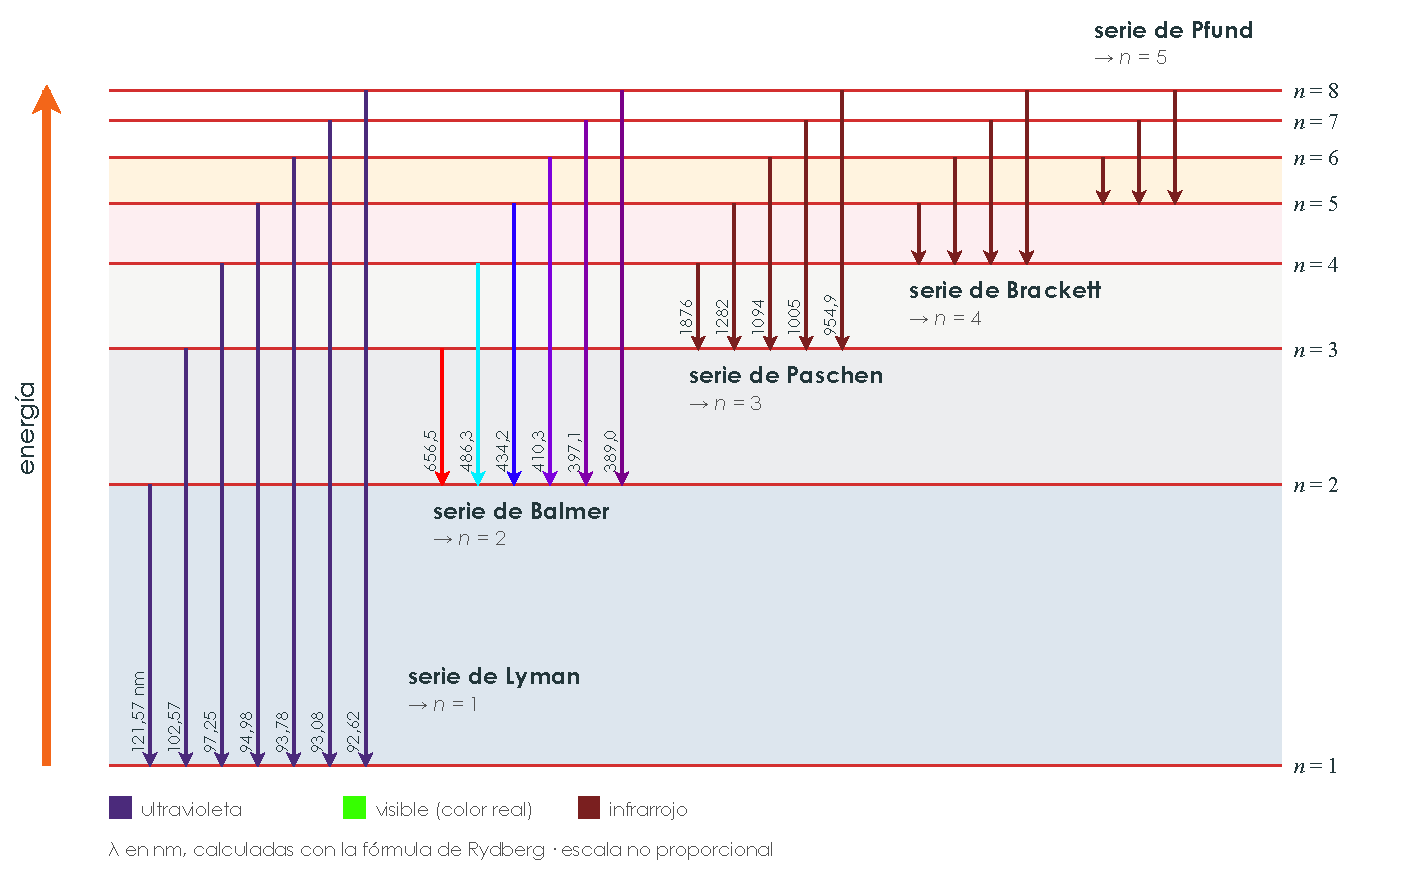
\includegraphics[width=0.9\linewidth]{FigurasSVG/UD1_Estructura_Atomica/pdf/UD1_11_series_espectrales.pdf}
    \caption{Series espectrales}
    \label{fig:series_espectrales}
\end{figure}

\subsection{Dualidad onda-corpúsculo. Principio de De Broglie}\label{subsec:dualidad-onda-corpusculo.-principio-de-de-broglie}
De Broglie recogió la idea de la naturaleza dual de la luz (se puede comportar como una onda y como un corpúsculo).

\begin{principio}[De Broglie]
    Las masas en movimiento se pueden comportar como ondas. Llegando a una expresión que relaciona la longitud de onda con la cantidad de movimiento según:
    \begin{centeredequation}
        \lambda = \dfrac{h}{p} \label{eq:debrolie}
    \end{centeredequation}
    Si tenemos en cuenta que \(p = m\ v\), la ecuación \eqref{eq:debrolie} quedaría como:
    \begin{centeredequation}
        \lambda = \dfrac{h}{mv} \label{eq:debrolie_desarrollada}
    \end{centeredequation}
    Siendo \(h\) la constante de Planck, \(v\) la velocidad de la partícula y \(m\) la masa de la partícula.
\end{principio}

\subsection{Principio de incertidumbre de Heisenberg}\label{subsec:principio-de-incertidumbre-de-heisenberg}

\begin{principio}[Principio de incertidumbre de Heisenberg]
    es imposible medir simultáneamente, y con precisión absoluta, el valor de dos variables conjugadas
\end{principio}

Este principio establece que la precisión de la medida es limitada.
Si tomamos una única coordenada para la posición y la cantidad de movimiento podemos establecer la siguiente expresión:

\begin{centeredequation}
    \Delta x \cdot \Delta p_x \geq \dfrac{h}{4\pi} \label{eq:heisenberg}
\end{centeredequation}
Donde:
\begin{gather*}
    \Delta x = \text{indeterminación en la posición}\separ
    \Delta p_x = \text{indeterminación en el impulso}\separ
    h ( \text{Constante de Plank}) = \SI{6.63e-34}{\joule\s}
\end{gather*}


\section{Números cuánticos}\label{sec:numeros-cuanticos}

Al resolver la ecuación de Schrödinger se observó que solo se permitían ciertas energías porque las funciones de onda dependían de tres variables que solo podían tomar unos valores discretos.
Estas variables son los \textbf{número cuánticos} $\mathbf{n, l\; y\; m}$.
Posteriormente, \textbf{Paul Adrien Murice Dirac} introdujo un número cuántico \textbf{spin \textit{s}}.

\begin{enumerate}[label=\numberballmDarkTeal]
        \item \textbf{\textit{n}} es el número cuántico principal, toma valores naturales excluidos el cero $\bm{n} = 1, 2, 3, 4 \dots$.
        Este número cuanto determina el nivel energético.
        Determina la extensión espacial, cuanto mayor sea el valor de $n$ mayor será el orbital.
        \item \textbf{\textit{l}} es el número cuántico secundario o azimutal, toma valores $ l = 0 \dots n-1$.
        Determina la forma del orbital atómico.
        Siguiendo la terminología espectroscopísta, los orbitales se designan como:
        \begin{enumerate}
            \item \textit{l} = 0.
            Orbital \blueremark{s} (sharp).
            Son esféricos.
            \begin{figure}[H]
                \centering
                % [FIGURA ORIGINAL] \includegraphics[scale=1]{images/imagesUD1EstructuraAtomica/UD1_Teoria/orbital_s}
                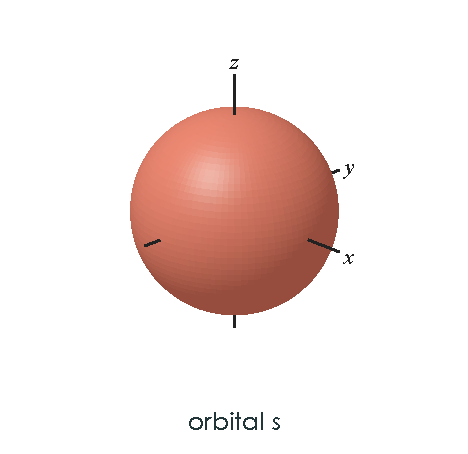
\includegraphics[width=0.3\linewidth]{FigurasSVG/UD1_Estructura_Atomica/pdf/UD1_12_orbital_s.pdf}
                \caption{Orbital \(\bm{s}\)}
                %\label{fig:}
            \end{figure}
            \item \textit{l} = 1.
            Orbital \blueremark{p} (principal).
            Presentan dos lóbulos idénticos a lo largo de un eje.
            La unión de ambos lóbulos coinciden con el núcleo atómico.
            Tenemos tres orbitales tipo $p$.  $p_x$,  $p_y$,  $p_z$.
            Cada uno de ellos llevará asociado un valor al número cuanto $m$ ($m=-1, m= 0, m=+1$).
            \begin{figure}[H]
                \centering
                % [FIGURA ORIGINAL] \includegraphics[scale=0.6]{images/imagesUD1EstructuraAtomica/UD1_Teoria/orbital_p}
                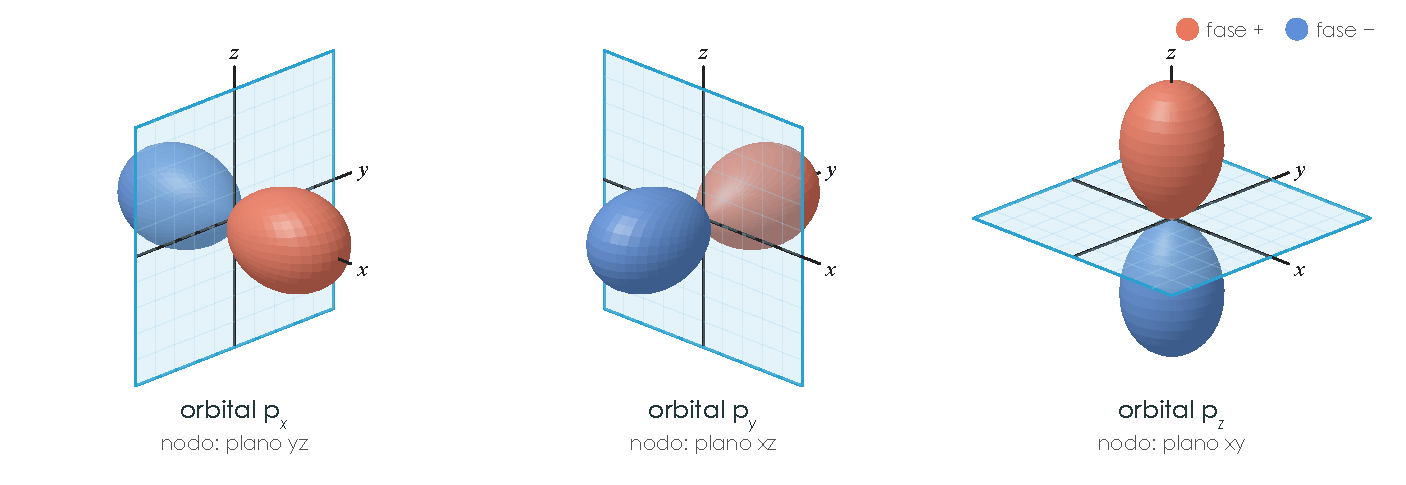
\includegraphics[width=0.9\linewidth]{FigurasSVG/UD1_Estructura_Atomica/pdf/UD1_13_orbitales_p.pdf}
                \caption{Orbitales \(\bm{p}\)}
                %\label{fig:}
            \end{figure}

            \item \textit{l} = 2.
            Orbital \blueremark{d} (diffuse).
            Están formados por lóbulos aunque más complejos.Los tenemos cuando $n\geq 3$.
            Hay 5 tipos de orbitales $d$. $d_{xy},\;d_{xz},\;d_{yz},\;d_{z^2},\;d_{x^2-y^2}$.
            Los valores asociados para el orbital $m$ serán ($m=-2, m=-1, m= 0, m=+1,m=+2$).

            \begin{figure}[H]
                \centering
                % [FIGURA ORIGINAL] \includegraphics[scale=0.6]{images/imagesUD1EstructuraAtomica/UD1_Teoria/orbital_d}
                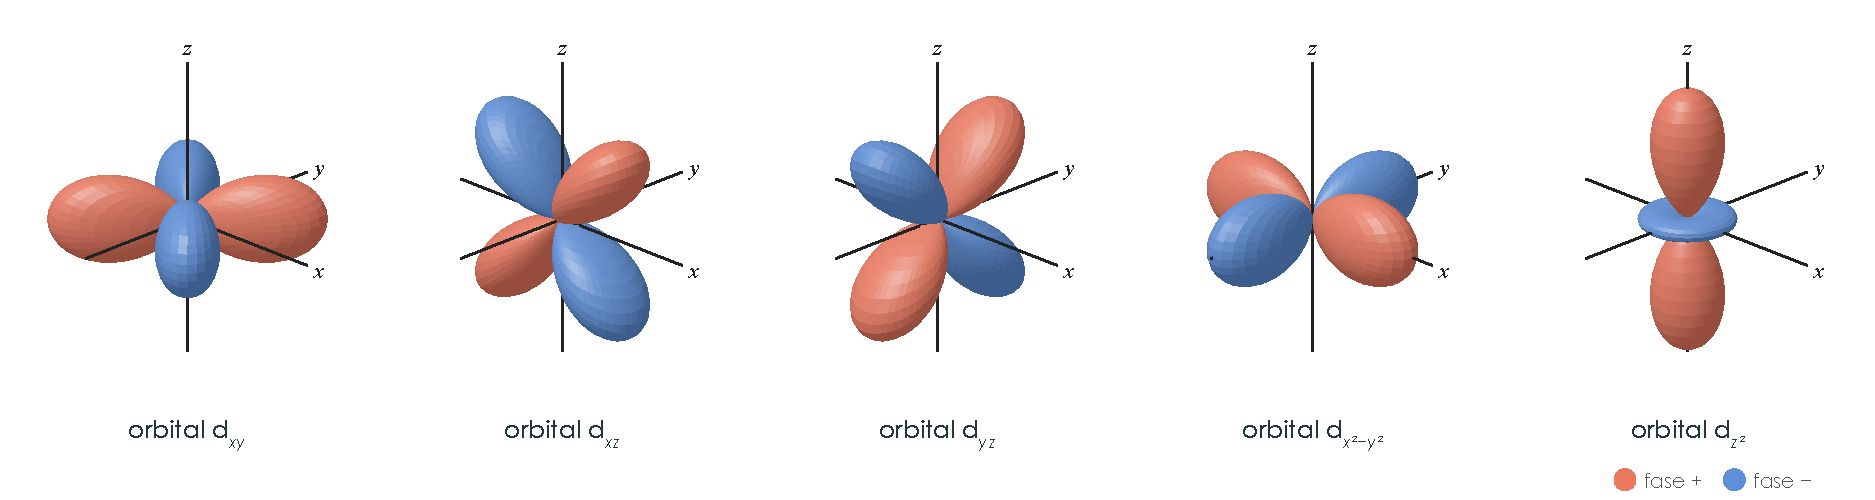
\includegraphics[width=1.0\linewidth]{FigurasSVG/UD1_Estructura_Atomica/pdf/UD1_14_orbitales_d.pdf}
                \caption{Orbitales \(\bm{d}\)}
                %\label{fig:}
            \end{figure}

            \item \textit{l} = 3.
            Orbital \blueremark{f} (fundamental).
            Los tenemos cuando $n\geq 4$.
            Tienen un aspecto multilobular.
            Existen 7 tipos de orbitales $f$ (que corresponden $m=-3, m=-2, m=-1, m= 0, m=+1,m=+2, m=+3$).

            \begin{figure}[H]
                \centering
                % [FIGURA ORIGINAL] \includegraphics[scale=0.7]{images/imagesUD1EstructuraAtomica/UD1_Teoria/orbitalesf}
                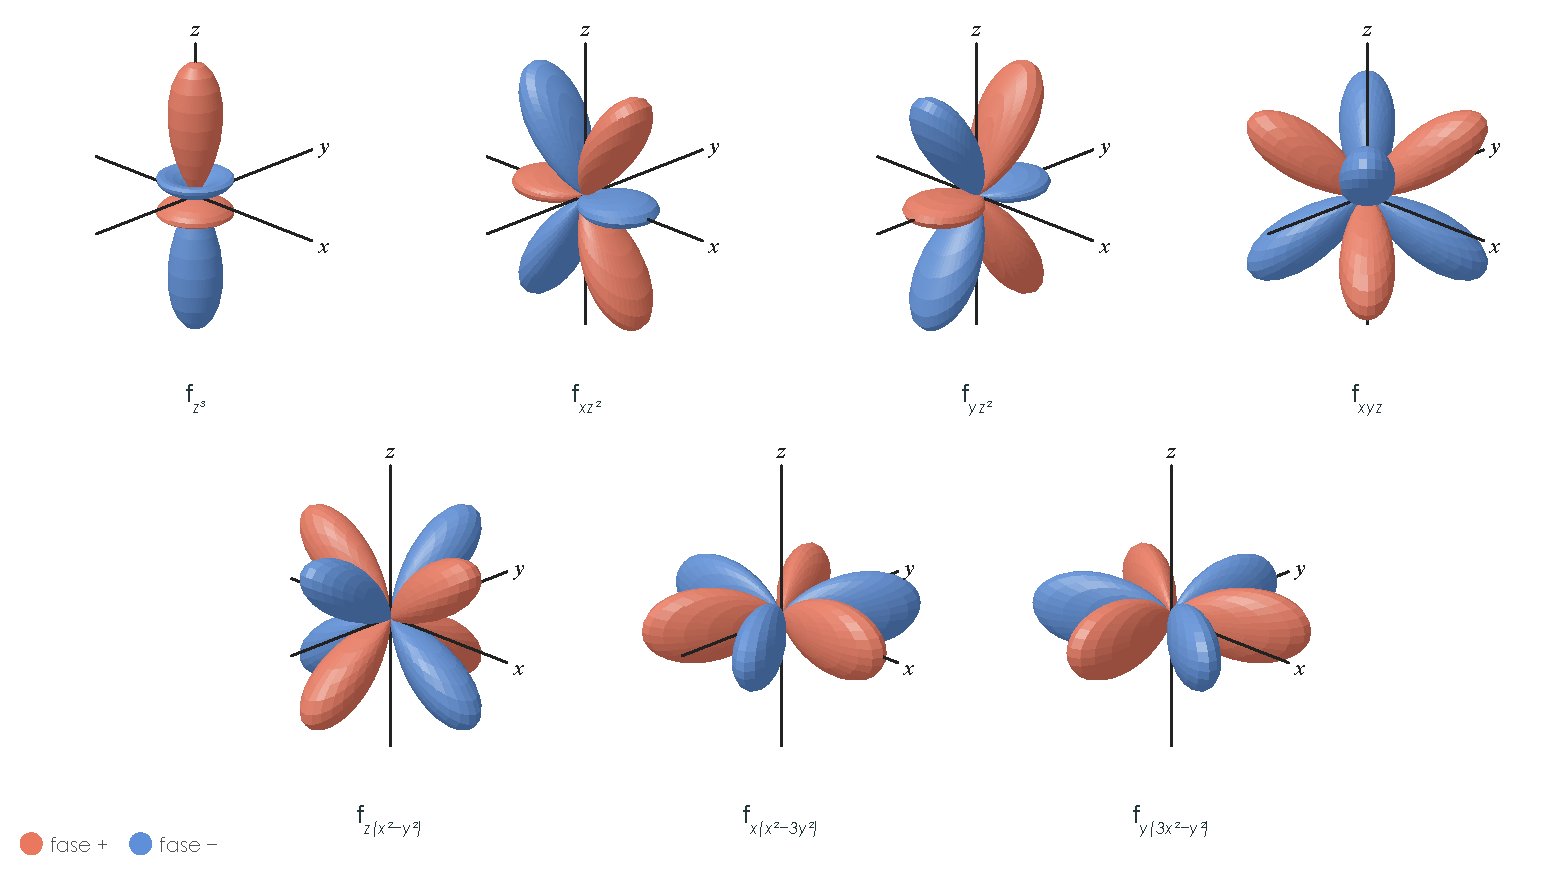
\includegraphics[width=0.9\linewidth]{FigurasSVG/UD1_Estructura_Atomica/pdf/UD1_15_orbitales_f.pdf}
                \caption{Orbitales \(\bm{f}\)}
                %\label{fig:}
            \end{figure}

        \end{enumerate}
        \item \textbf{\textit{m}} es el número cuántico magnético, toma valores desde $-l \dots 0 \dots +l$.
        Determina la orientación espacial del orbital.
        \item \textbf{\textit{s}} es el número cuántico de spin.
        Solo toma los valores $-\frac{1}{2}$ y $+\frac{1}{2}$.
        Determina el giro del electrón sobre sí mismo.
\end{enumerate}
% \begin{figure}
%     \centering
%     \includegraphics[scale=1]{forma_orbitales.png}
%     \caption{Forma de los orbitales atómicos}
%     \label{fig:forma_orbitales}
% \end{figure}

\subsection{Orden energético para los electrones de los átomos}\label{subsec:orden-energetico-para-los-electrones-de-los-atomos}

\subsubsection{Diferentes niveles de energía}

La energía de cada electrón depende de los cuatro números cuánticos.
Según el valor de estos podemos definir, el nivel, el subnivel y el orbital.
\begin{enumerate}[label=\numberballmDarkTeal]
        \item \textbf{Nivel}.
        Los electrones con el mismo número cuántico principal $n$ se dicen que forman parte de la misma capa o nivel energético.
        \item \textbf{Subnivel}.
        Cada capa o nivel tiene a su vez subcapas o subniveles.
        Así se dice que en el nivel $n=3$ se encuentran los subniveles $3s\;(l=0)$, $3p\;(l=1)$, $3d\;(l=2)$
        \item \textbf{Orbital} Aquellos electrones que tienen los mismos números cuánticos $n$ y $l$ pero diferente $m$ se dice que pertenecen al mismo orbital.
        En cada orbital caben como máximo dos electrones que se diferencia por el número cuántico de spin $s$.
        En cada subnivel $l$ hay $2l+1$ orbital, con lo que en un nivel $n$ caben $2n^2$ electrones.
\end{enumerate}

Para determinar la energía de cada orbital, se establece que los orbitales con una suma del número cuántico \(n\) y el \(l\) (\(n + l\)) más bajo, tendrán menos energía.
Otra manera de determinarlo es siguiendo el orden de llenado según el diagrama de Moeller

\subsection{Distribución electrónica}\label{subsec:distribucion-electronica}

La distribución electrónica nos indica como se alojan los diferentes electrones en sus correspondientes orbitales y para ello siguen las siguientes reglas:

\begin{enumerate}[label=\numberballmDarkTeal]
        \item \textbf{Principio de exclusión de Pauli}: Un átomo no puede tener 2 electrones con los mismos 4 números cuánticos.
        En un orbital puede haber como máximo 2 electrones.
        \item \textbf{Principio de mínima energía}: los electrones se colocan en el orbital de menos energía que esté disponible.
        El orden de la energía está determinado por la suma dé $n + l$.
        Si dos orbitales tienen el mismo valor de $n+l$ el de menor energía será aquel que tenga menor valor dé $n$.

        \item \textbf{Principio de máxima multiplicidad de Hund}: a igualdad de los principios anteriores, la configuración más estable es la que permite el máximo desapareamiento de los electrones.
\end{enumerate}

El orden de llenado también se puede seguir según el diagrama de Moeller.
\begin{figure}[H]
    \centering
    \begin{tikzpicture}[>=stealth, font=\sffamily\LARGE\bfseries]

        % --- Configuración de Colores ---
        \definecolor{mygreen}{RGB}{0, 128, 0}
        \definecolor{myblue}{RGB}{91, 155, 213}

        % --- Dibujado de los Subniveles ---
        % Separación horizontal (2.2) y vertical (1.2) para que las diagonales sean perfectas
        \newcommand{\subnivel}[5]{
            \node (n#3#4) at (#1*2.2, -#2*1.2) {#3\textcolor{mygreen}{\textit{#4}}\textsuperscript{\textcolor{red}{#5}}};
        }

        % Columna s (x=0)
        \foreach \n in {1,...,7} \subnivel{0}{\n}{\n}{s}{2};
        % Columna p (x=1)
        \foreach \n in {2,...,7} \subnivel{1}{\n}{\n}{p}{6};
        % Columna d (x=2)
        \foreach \n in {3,...,7} \subnivel{2}{\n}{\n}{d}{10};
        % Columna f (x=3)
        \foreach \n in {4,...,7} \subnivel{3}{\n}{\n}{f}{14};

        % --- Dibujado de las Flechas Diagonales ---
        % Estilo: pasan por el centro, color azul, y se extienden 0.8cm hacia atrás y 1cm hacia adelante
        \tikzset{flecha/.style={myblue, very thick, *->, shorten <=-0.8cm, shorten >=-1cm}}

        % Para flechas que cruzan varios nodos (del centro del primero al centro del último)
        \draw[flecha] ($(n2p.center)+(1.5,0.7)$) -- (n3s.center);
        \draw[flecha] ($(n3p.center)+(1.5,0.7)$) -- (n4s.center);
        \draw[flecha] ($(n3d.center)+(1.5,0.7)$) -- (n5s.center);
        \draw[flecha] ($(n4d.center)+(1.5,0.7)$) -- (n6s.center);
        \draw[flecha] ($(n4f.center)+(1.5,0.7)$) -- (n7s.center);
        \draw[flecha] ($(n5f.center)+(1.5,0.7)$) -- (n7p.center);
        \draw[flecha] ($(n6f.center)+(1.5,0.7)$) -- (n7d.center);

        % Para las flechas de un solo nodo (1s, 2s y 7f), definimos una dirección manual
        % para que mantengan el mismo ángulo que las demás.
        \draw[flecha] ($(n1s.center)+(1.5,0.7)$) -- (n1s.center);
        \draw[flecha] ($(n2s.center)+(1.5,0.7)$) -- (n2s.center);
        \draw[flecha] (n7f.center) ++(1.5,0.8) -- (n7f.center);

    \end{tikzpicture}
    \caption{Moeller Diagram}
    \label{fig:diagrama_moeller}
\end{figure}
%\begin{figure}[H]
%    \centering
%    \includegraphics[scale=.5]{images/imagesUD1EstructuraAtomica/UD1_Teoria/diagrama_moeller}
%    \caption{Diagrama de Moeller}
%    \label{fig:diagrama_de_moeller}
%\end{figure}

Según estos principios, si un \el{} se encuentra en su estado fundamental estará, por tanto, en un estado de mínima energía.
Si ese \el{} se encuentra excitado, estará, en consecuencia, en un estado de mayor energía mientras que si un \el{} se encuentra en un estado prohibido será un estado imposible desde el punto de vista cuántico incumpliendo el principio de exclusión de Pauli.

\subsubsection{Excepciones al orden de llenado y justificación de los estados de oxidación.}

Hay excepciones a las reglas de llenado como por el ejemplo:
\begin{itemize}
    \item \elementsymbol{24}(Z=\atomicnumber{Cr}) \elconf{Cr}
    \item \elementsymbol{29}(Z=\atomicnumber{Cu}) \elconf{Cu}
    \item \elementsymbol{47}(Z=\atomicnumber{Ag}) \elconf{Ag}
    \item \elementsymbol{79}(Z=\atomicnumber{Au}) \elconf{Au}
    \item \elementsymbol{42}(Z=\atomicnumber{Mo}) \elconf{Mo}
\end{itemize}

Estas excepciones se deben a que la configuración más estable es aquella que tenga los subniveles \textbf{llenos} / \textbf{capa cerrada} es decir aquellos que tienen como configuración electrónica \(ns^2\;  np^6\) a excepción del He (\(2s^2\)) o \textbf{semillenos} / \textbf{semicapa cerrada} es decir aquellos que tienen como configuración electrónica \(ns^1, \; np^3, \; nd^5, \; nf^7, \;\)

Los estados de oxidación de los elementos se pueden predecir teniendo en cuenta la configuración electrónica, el elemento perderá o ganará electrones de manera que adquiera la configuración electrónica más estable, siendo esta la de gas noble o bien con capas llenas o semillenas.

